\RequirePackage{iftex}
\ifXeTeX
\IfFileExists{/System/Library/Fonts/Supplemental/Times New Roman.ttf}{
\DeclareFontFamily{TU}{ptm}{}
\DeclareFontShape{TU}{ptm}{m}{n}{<->"Times New Roman:letterspace=0"}{}
\DeclareFontShape{TU}{ptm}{m}{it}{<->"Times New Roman Italic"}{}
\DeclareFontShape{TU}{ptm}{bx}{n}{<->"Times New Roman Bold"}{}
\DeclareFontShape{TU}{ptm}{b}{n}{<->"Times New Roman Bold"}{}
\DeclareFontShape{TU}{ptm}{m}{sc}{<->"Times New Roman"}{}
\DeclareFontShape{TU}{ptm}{bx}{it}{<->"Times New Roman Bold Italic"}{}
\DeclareFontShape{TU}{ptm}{b}{it}{<->"Times New Roman Bold Italic"}{}
}{}
\fi
\ifXeTeX
\IfFileExists{/System/Library/Fonts/Supplemental/Arial.ttf}{
\DeclareFontFamily{TU}{phv}{}
\DeclareFontShape{TU}{phv}{m}{n}{<->"Arial"}{}
\DeclareFontShape{TU}{phv}{m}{it}{<->"Arial Italic"}{}
\DeclareFontShape{TU}{phv}{bx}{n}{<->"Arial Bold"}{}
\DeclareFontShape{TU}{phv}{b}{n}{<->"Arial Bold"}{}
\DeclareFontShape{TU}{phv}{b}{it}{<->"Arial Bold Italic"}{}
\DeclareFontShape{TU}{phv}{bx}{it}{<->"Arial Bold Italic"}{}
}{}
\fi
\documentclass[11pt,onecolumn,conference,letterpaper]{IEEEtran}
\usepackage[left=.96in,right=.96in,top=.91in,bottom=.86in,headheight=15pt,headsep=17pt]{geometry}
\usepackage{amsmath,amssymb,booktabs,array,graphicx,xcolor,cite}
\usepackage[hidelinks]{hyperref}
\usepackage{microtype}
\definecolor{maroon}{HTML}{801939}
\definecolor{charcoal}{HTML}{272927}
\definecolor{quiet}{HTML}{56575A}
\definecolor{warm}{HTML}{F7F4ED}
\definecolor{gold}{HTML}{EDB62F}
\hypersetup{pdftitle={ReelRank: Which Title Should Come First?},pdfauthor={Usman Mehboob Mohammed, Moin Palekar, Omkar Rajesh Hundekari, Aryan Tripathi, Badri Sri Vaishnavi Yeluri, Arya Ravindra Patil}}
\urlstyle{same}
\setlength{\emergencystretch}{1.3em}
\setlength{\parindent}{0pt}
\setlength{\parskip}{5.5pt}
\renewcommand{\baselinestretch}{1}
\raggedbottom
\makeatletter
\def\ps@coursepaper{%
  \def\@oddhead{\vbox{\hbox to \textwidth{\color{maroon}\sffamily\bfseries\footnotesize REELRANK\hfil\color{quiet}\normalfont\sffamily\footnotesize ARIZONA STATE UNIVERSITY\quad / \quad CSE 575}\vspace{4pt}\color{maroon}\hrule height .4pt}}%
  \def\@evenhead{\@oddhead}%
  \def\@oddfoot{\hfill{\color{quiet}\sffamily\small\thepage}}%
  \def\@evenfoot{\@oddfoot}}
\makeatother
\newcommand{\topic}[1]{\par\medskip{\noindent\color{maroon}\sffamily\bfseries\large #1\par}\smallskip}
\newcommand{\rowhead}[1]{{\sffamily\small\bfseries #1}}
\newcommand{\pull}[2]{\par\smallskip\noindent{\setlength{\fboxsep}{10pt}\colorbox{warm}{\begin{minipage}{\dimexpr\linewidth-2\fboxsep\relax}\raggedright
{\sffamily\bfseries\color{maroon}#1}\hspace{.45em}#2\end{minipage}}}\par\smallskip}
\newcommand{\art}[3]{\par\smallskip\noindent\begin{minipage}{\linewidth}\centering
\includegraphics[width=.99\linewidth,height=2.81in,keepaspectratio]{figures/choice_pitch_#1.pdf}\par\vspace{4pt}
\raggedright\refstepcounter{figure}{\footnotesize{\sffamily\bfseries\color{maroon}Fig. \thefigure.}\enspace #2\par}\label{#3}
\end{minipage}\par\smallskip}
\newcommand{\tabletitle}[1]{\par\medskip\refstepcounter{table}{\noindent\small\sffamily{\bfseries\color{maroon}TABLE \Roman{table}.}\enspace #1\par}\vspace{1pt}}
\newcommand{\note}[1]{\par{\noindent\small\color{quiet}#1\par}}
\newcommand{\pnum}[2]{\begin{minipage}[t]{.30\linewidth}\raggedright{\fontsize{28}{30}\selectfont\bfseries\sffamily\color{maroon}#1}\par\vspace{3pt}{\sffamily\small #2\par}\end{minipage}}
\title{ReelRank: Which Title Should Come First?}
\author{\IEEEauthorblockN{Usman Mehboob Mohammed, Moin Palekar, Omkar Rajesh Hundekari,\\
Aryan Tripathi, Badri Sri Vaishnavi Yeluri, and Arya Ravindra Patil}
\IEEEauthorblockA{Arizona State University\quad / \quad CSE 575, Statistical Machine Learning}}
\begin{document}
\pagestyle{coursepaper}
\maketitle
\thispagestyle{coursepaper}
\begin{abstract}
People can choose only from the titles they are shown. ReelRank uses that simple observation to decide which movie or book to recommend first. It learns how a person's earlier selections differ from the mix of titles they were offered, then scores the next ten titles. On 5,510 lists from 349 held-out participants, ReelRank placed a title the participant had marked for consideration first on 2,920 lists. UserKNN, the strongest of the six released SM-RS recommendation engines on this metric, did so on 2,578. That is 342 additional correct first choices, or about six more per 100 lists (6.21 percentage points, paired 95\% interval 4.83 to 7.55). Implicit matrix factorization led the released methods on whole-list nDCG@10 at 0.6561. ReelRank reached 0.6850. A tuned LambdaMART ranker using the same 352 features achieved 2,882 first hits. ReelRank led by 0.69 points (95\% interval $-0.36$ to 1.75). On 376,471 news lists, a separate frozen ReelRank model placed a clicked headline first on 2,103 more lists than an equal-weight average of nine public neural checkpoints. Both studies measure agreement with recorded choices.
\end{abstract}

\section{Introduction}
A viewer picks two thrillers. Does that tell us they like thrillers? If every film on the screen was a thriller, genre tells us little about the choice. If those two films were the only thrillers in a varied lineup, choosing both tells us more. A recommender that saves only the two picks loses that distinction.

This question matters at the top of a list. A service can retrieve ten plausible titles and still put the one a viewer wants near the bottom. Once a service has retrieved ten plausible titles, which one should it put first? Movies and books give us an unusually direct way to test it. In the SM-RS study, people saw actual lists and marked what they would consider watching or reading that evening~\cite{smrs,smrs2}.

Personalized reranking is well established~\cite{pei}. Choice models also recognize that the alternatives on offer affect what a selection means~\cite{choice}. ReelRank estimates that contrast for each participant and combines it with catalog features and six published recommendation signals. We compare the resulting system with every individual ranking method released for SM-RS Task 3. We also fit an external LambdaMART learner using the same inputs and supervision. The released engines show what each established method can achieve on its own. The feature-matched learner tests whether our scoring algorithm adds anything when both methods already have the same evidence.

\noindent\begin{minipage}[c]{.51\linewidth}
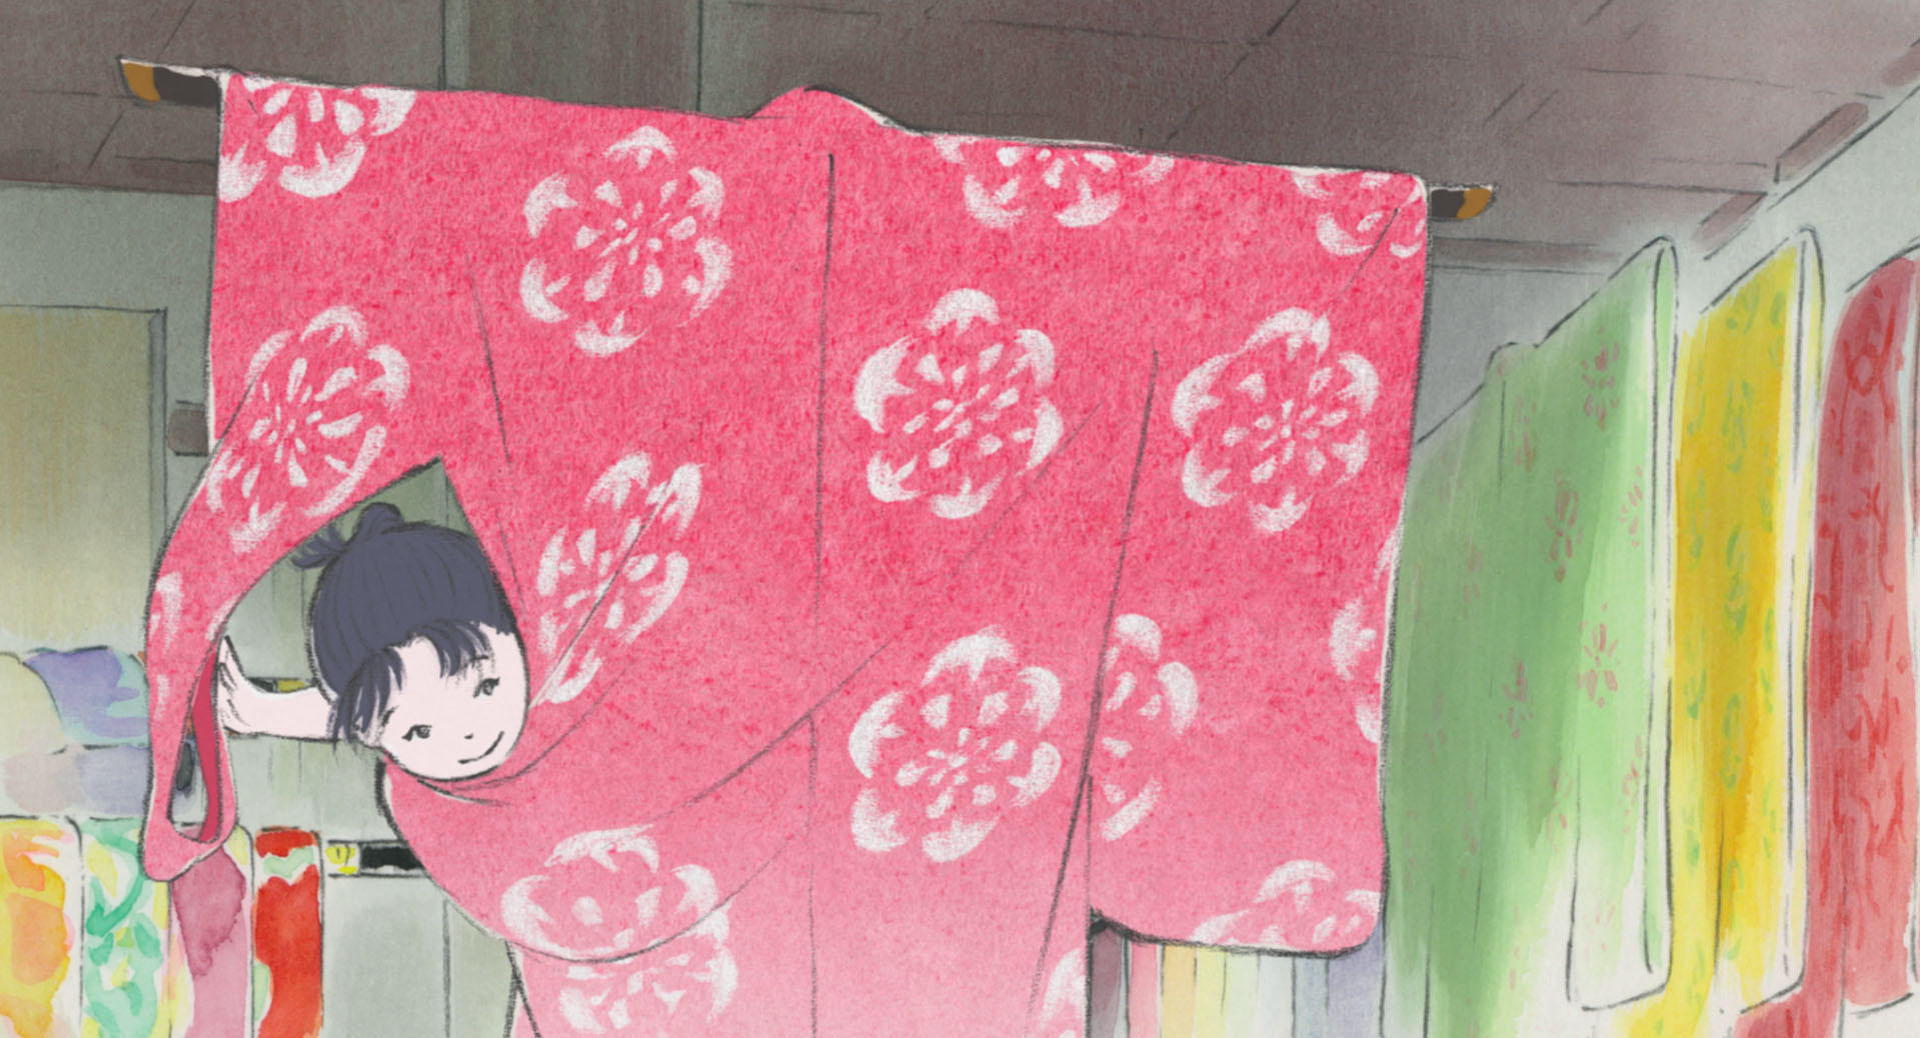
\includegraphics[width=\linewidth]{figures/choice_pitch_kaguya.jpg}
\end{minipage}\hfill\begin{minipage}[c]{.45\linewidth}\raggedright
{\color{maroon}\sffamily\bfseries One viewer's choice}\par\smallskip
\textit{The Tale of the Princess Kaguya} (2013) was the only film one participant marked on a list of ten. The original screen placed it sixth. ReelRank put it first.
\par\smallskip{\scriptsize Film still \textcopyright\ 2013 Isao Takahata, Riko Sakaguchi/Studio Ghibli, NDHDMTK. \href{https://www.ghibli.jp/works/kaguyahime/}{Studio Ghibli film archive}.}
\end{minipage}\par\smallskip
\clearpage
\section{Problem description}
\topic{What counts as getting the first title right?}
Each observation is one ten-title list shown to one participant. The person could mark several titles, one title, or none. We replay the list using only information available before it was displayed. A \emph{first-position hit} occurs when the model's first title is among the person's recorded choices. Every list counts once. A list on which the participant marked nothing gives every model a miss.

\art{opportunity}{An illustrative choice history. Seeing what else was offered helps the model interpret a selection. The example explains the input. The scores in the results section come from the recorded study.}{fig:opportunity}

\topic{Reading one prediction}
Consider the \textit{Princess Kaguya} example on the opening page. The locations below are ranks of the same film among the same ten candidates. The first-position metric gives a hit whenever the marked title leads the list. A title can move closer to the top and still fall short on this metric.

\noindent\pnum{6th}{Recorded display}\hfill\pnum{4th}{Published UserKNN}\hfill\pnum{1st}{Personalized ReelRank}\par
\smallskip
We chose this example after scoring to show what a rank change looks like. We use all 5,510 held-out lists to estimate how frequently each method succeeds. Section~\ref{sec:results} gives those counts for the complete cohort.

\topic{Where the judgments come from}
SM-RS 2.0 supplies the displayed items and selections~\cite{smrs2,package}. MovieLens 25M and goodbooks-10k supply catalog information, including tags and rating statistics~\cite{ml25,mlhistory,goodbooks}. A historical rating can describe a film's broad appeal. Only the participant's selection on this particular list determines whether the prediction was right. A selection means the person would consider the title that evening. The study did not follow them through to a completed film or book.

\clearpage
\section{Methodology}
\topic{Learn from the titles a person could have chosen}
Before the next list appears, ReelRank can draw on two kinds of history. The first contains distinct titles already offered to the person. The second contains earlier titles they actually selected. We add an offered title at display time and a selected title only after its response. If an earlier event shares the new display's timestamp, we leave it out. The current selections and original screen positions never enter the prediction.

\art{method}{The reranker operates on a fixed set of ten candidates. Earlier offers and selections describe the viewer. Catalog information and the existing engines describe each candidate. The two fitted scoring models produce a new order.}{fig:method}

\topic{Estimate a preference from limited evidence}
Each title has numerical features describing what it resembles. Collaborative features place together titles with similar rating patterns. Tags describe content. Catalog descriptors capture characteristics such as a film's release year and popularity. For each of these three representations we compare the average selected title with the average offered title. A candidate close to that difference can fit the person's choices even if it is less broadly appealing.

Some histories are short or narrow. The model uses \emph{shrinkage} to limit how strongly an uncertain direction can influence the score. It also measures whether a candidate resembles the nearest earlier selections or the most recent ones. Until there is evidence from both offers and selections, the new personal features are zero. Population signals still provide a ranking.

\topic{Combine personal and population evidence}
ReelRank uses scores from the released models for popularity, item associations, matrix factorization, user neighborhoods and two autoencoders. It combines their six rankings with catalog features, candidate coordinates and the viewer's historical choices and offers. A conditional logit compares candidates within the list. Gradient-boosted trees allow the value of a signal to change with other features. After scaling both scores within the list, the development data favored an equal mixture.

\clearpage
\topic{How we tested the algorithm}
The 435 participants supplied 6,892 ten-title displays. We assigned whole people to development or evaluation. Every model ranked the same ten titles on each evaluation display, which makes the comparisons paired. The model can learn from a held-out participant's own past responses while making a prediction for that participant. Their comparison labels never enter population-model training or tuning for this extension.

\tabletitle{Who contributed to the main comparison}
\begin{center}\renewcommand{\arraystretch}{1.28}\begin{tabular}{@{}lrrp{2.7in}@{}}\toprule
\rowhead{Cohort} & \rowhead{People} & \rowhead{Lists} & \rowhead{Use in the experiment}\\\midrule
Development & 86 & 1,382 & Fit the model and select the score mixture.\\
Held out & 349 & 5,510 & Score every model on the same lists.\\
\bottomrule\end{tabular}\end{center}

Within development, four folds separated participants. We compared four gradient-boosting weights, from 25\% to 100\% in steps of 25 points. The selection rule favored the most correct first choices, then the highest whole-list ranking score to break a tie. After choosing the equal mixture we froze the recipe. The comparison participants were excluded from this fit, although aggregate outcomes on their public cohort had been examined in earlier work. The first comparator family comes from the SM-RS release. The second is LightGBM 4.6.0 LambdaMART trained on all 352 input features with identical labels and the same four participant folds~\cite{lgb,burges}. Its development grid included 12 settings. The chosen configuration used 31 leaves, 200 trees and a ranking truncation level of three. We also reproduced the separate published Task 3 protocol to check that its scores could be recovered (Appendix B).

\topic{Three ways to read a recommendation list}
\textbf{First-position hit rate (Hit@1).} Imagine revealing only the first title on every list. How often would a marked title be visible? There were 634 held-out lists with no marked titles. Keeping those lists makes 5,510 the denominator for every method.

\textbf{Ranking quality (nDCG@10).} This score gives a marked title more credit near the top. Each list is compared with its own ideal arrangement, where all its marked titles appear first. A value of one is a perfect ordering on a nonempty list. An empty selection receives zero.

\textbf{Precision at five (P@5).} Count how many of the top five titles the participant marked and divide by five. A list with two marked titles in the top five contributes 0.4. This metric can distinguish two rankings that put the same title first.

\topic{Count the uncertainty by person}
A person often supplied several related lists. For the 95\% intervals we resampled entire participants 5,000 times, kept their lists together and recalculated the paired differences. The main estimate gives every list equal weight. The intervals describe variation across people conditional on the fitted systems. Each interval concerns a single comparison and does not adjust for selecting a leading reference method. They do not account for a new catalog, a different user population or model retraining.

\clearpage
\section{Results}\label{sec:results}
\topic{The lead title matched a participant's choice on 2,920 lists}
We tested the recorded order and all six recommendation engines supplied for SM-RS Task 3. UserKNN led these seven reference rankings on first-position hits. It predicts from the behavior of similar users, following the neighborhood approach to collaborative filtering~\cite{grouplens}. Across 5,510 held-out lists it put a marked title first 2,578 times (46.79\%). ReelRank reached 2,920 (52.99\%). On 777 lists ReelRank placed a selected title first where UserKNN missed, and on 435 the reverse occurred. The 342 net additional correct placements amount to 6.21 percentage points, with a participant-paired 95\% interval of 4.83 to 7.55 points.

\art{evidence}{UserKNN is the strongest single SM-RS engine on Hit@1. LambdaMART is the stronger, feature-matched external learner. Points and confidence intervals show the increase in Hit@1 when the complete ReelRank system scores the same ten titles.}{fig:evidence}

\topic{Did the whole list improve too?}
Among the six released engines, a different method led the two whole-list measures. Implicit matrix factorization learns a compact representation from user-item interaction patterns~\cite{hu}. Its nDCG@10 was 0.6561, the highest among these seven reference rankings. ReelRank reached 0.6850, an improvement of 0.0289 (95\% interval 0.0240 to 0.0337). Implicit matrix factorization led the same reference rankings on precision at five, at 0.3881. ReelRank reached 0.4145, a gain of 0.0264 (0.0224 to 0.0304). Appendix A gives every comparator, including the original displayed order.

\topic{A harder comparison with identical inputs}
LambdaMART scored 2,882 first hits. ReelRank scored 38 more. The difference of 0.69 points had a 95\% interval from $-0.36$ to 1.75. Whole-list nDCG@10 was 0.6824 for LambdaMART and 0.6850 for ReelRank. The interval for this difference also included zero. Thus the gain over the best single released model is clear, while these data do not establish a reliable main-cohort advantage over the stronger supervised comparator.

\clearpage

\topic{Where the 342 additional correct first choices came from}
A service might do well by preserving the original first title, which the participant saw first when making the choice. To see whether the gain was concentrated there, we traced each correct prediction back to the selected title's original screen position. This is a post hoc interpretation of the measured rankings.

\art{positions}{Net change in correct first choices against UserKNN, grouped by the title's position in the recorded interface. Each correct prediction contributes to just one position group.}{fig:positions}

Among titles originally at positions two through ten, ReelRank recorded 2,400 correct leads, compared with 2,132 for UserKNN. Of the net gain of 268 from those positions, 124 came from positions two through five and 144 from positions six through ten. Another 74 came from titles originally shown first. Together the three groups account for all 342 net additional correct predictions. The original order may itself have influenced what people marked.

\topic{How many lists have a marked title near the top?}
On the 4,876 nonempty lists, the first marked title appeared at position 2.06 on average under ReelRank and 2.35 under UserKNN. The table below counts every held-out list, including empty selections. The difference was largest at the first position, the decision the model was trained to improve.

\tabletitle{Lists containing a marked title within the indicated number of positions}
\begin{center}\renewcommand{\arraystretch}{1.23}\begin{tabular}{@{}lrrrr@{}}\toprule
\rowhead{Positions examined}&\rowhead{One}&\rowhead{Two}&\rowhead{Three}&\rowhead{Five}\\\midrule
UserKNN & 2,578 & 3,407 & 3,896 & 4,414\\
ReelRank & 2,920 & 3,704 & 4,135 & 4,526\\
Net gain & 342 & 297 & 239 & 112\\\bottomrule\end{tabular}\end{center}
\note{All 5,510 held-out lists contribute. This measures recorded positions. No viewing time or time saved was measured.}

\clearpage

\topic{Does the result depend on who is in the test set?}
On the 4,088 movie lists, 52.64\% had a marked film first under ReelRank and 46.70\% did under UserKNN. On the 1,422 book lists, the corresponding rates were 54.01\% and 47.05\%. Thus the pooled gain includes improvements in both domains. These rates describe two different groups who were offered different catalogs.

In a separate five-fold analysis that allowed all 435 participants a turn in evaluation, ReelRank reached 54.19\% and UserKNN reached 46.89\% on the 6,892 lists. The difference was 7.30 percentage points (95\% interval 6.17 to 8.45). The five folds give another view of the same public study. They do not constitute an independent new population.

\topic{Can a model fitted on earlier people rank for later arrivals?}
We chose a calendar cutoff, trained on the 229 participants who finished before it and evaluated the 131 who began after it. The split excluded 75 participants whose sessions crossed the boundary. All 229 earlier participants were in the movie study. Among the later participants, 30 were in movies and 101 were in books. The test therefore changes both calendar period and catalog mix. We refit the models on the early participants with settings selected in the main development cohort. That cohort was not restricted to this earlier calendar period. This is a time-separated sensitivity check on fitted weights, rather than a fully prospective tuning test.

\tabletitle{The later-participant test used all 2,358 eligible lists}
\begin{center}\renewcommand{\arraystretch}{1.27}
\begin{tabular}{@{}lrrr@{}}\toprule
\rowhead{Ranker}&\rowhead{First hits}&\rowhead{Hit@1}&\rowhead{nDCG@10}\\\midrule
LambdaMART & 1,113 & 47.20\% & 0.6675\\
Implicit matrix factorization & 1,146 & 48.60\% & 0.6868\\
User nearest neighbors & 1,185 & 50.25\% & 0.6871\\
Personalized ReelRank & \textbf{1,186} & \textbf{50.30\%} & \textbf{0.6952}\\
\bottomrule\end{tabular}\end{center}

The difference in first-position hit rate versus UserKNN was 0.04 points (95\% interval $-2.16$ to 2.21), effectively a tie. UserKNN also had the strongest released nDCG@10 on these later lists. ReelRank reached 0.6952 against 0.6871, with a paired interval on the difference that included zero. Against the independently tuned LambdaMART model, ReelRank placed a selected title first on 73 additional lists, a gain of 3.10 points (1.15 to 5.09). Implicit matrix factorization led the released methods on precision at five, at 0.4056 versus ReelRank's 0.4143.

\pull{What changes with the audience}{A 6.21-point first-position advantage on the main participant holdout shrank to one list in the later-participant sensitivity check. The mix of movie and book participants also changed.}

\clearpage

\topic{Can a reader's next click move closer to the top?}
Movies and books give us expressions of interest. News records which headlines people actually clicked. We tested the same first-position question on Microsoft's MIND data with a separately designed news ranker~\cite{mind}. The movie model and the news model have different inputs and fitted weights.

Our comparison uses public NewsReX checkpoints for NRMS, which learns from title text and reading history, NAML, which uses multiple article representations, and LSTUR, which combines long- and short-term reader interests~\cite{nrms,naml,lstur,newsrex}. We evaluate the complete MIND-large public validation file and also screen for identifiable overlap with MIND-small development. The screened cohort is a subset of full validation from the same service and date.

\tabletitle{How often did a clicked headline rank first?}
\begin{center}\renewcommand{\arraystretch}{1.23}\begin{tabular}{@{}lrrrr@{}}\toprule
&\multicolumn{2}{c}{\rowhead{259,161 screened lists}}&\multicolumn{2}{c}{\rowhead{376,471 validation lists}}\\
\rowhead{Method}&\rowhead{First hits}&\rowhead{nDCG@10}&\rowhead{First hits}&\rowhead{nDCG@10}\\\midrule
NAML / 456 & 50,235 & 0.4106 & 73,554 & 0.4131\\
Nine-model average & 51,555 & 0.4202 & 75,245 & 0.4226\\
ReelRank, matched training & 52,952 & 0.4245 & 77,348 & 0.4268\\
ReelRank, delayed feedback & 53,512 & 0.4297 & 78,190 & 0.4323\\
\bottomrule\end{tabular}\end{center}
\note{The external checkpoint shown led the nine individual checkpoints. We also averaged all nine checkpoints with equal weights. Appendix C lists the individual scores.}

\art{news}{Each point shows the gain for the matched frozen model against one external comparison. Horizontal lines show the paired 95\% intervals across reader accounts.}{fig:news}

\topic{What information is available when a headline is scored?}
ReelRank blends three NAML scores, an NRMS score and a local estimate of article popularity and reader affinity. For the frozen comparison, the local model used the same 149,117 training impressions as the NewsReX models and at most 50 articles of reading history. It received no same-day feedback. ReelRank recorded 77,348 first hits. It gained 3,794 over NAML seed 456 and 2,103 over the nine-model average. Against the average, that is 0.559 percentage points (95\% interval 0.462 to 0.655). Whole-list nDCG@10 also increased by 0.00428.

The delayed-feedback version also estimates article appeal using MIND-small impressions from earlier hours, with a full hour of reporting delay. When this score and the frozen model favor different first headlines, a logistic classifier chooses between them. This system placed a clicked headline first on 78,190 lists, 2,945 more than the nine-model average. It had access to newer information. These are historical clicks moved to the top. A randomized trial would measure changes in how often readers click. Appendix D gives the results for three additional methods fitted on full MIND-large training data.
\clearpage

\section{Conclusions and future work}
\topic{Keep the alternatives alongside the choices}
A recommendation service can learn from the titles on the screen when a viewer makes a choice. ReelRank turns that record into a personal preference estimate and combines it with six existing recommendation scores. Across 5,510 held-out lists, the complete ReelRank system recorded 342 more correct first choices than UserKNN and improved whole-list nDCG@10 by 0.0289 over implicit matrix factorization. A feature-matched LambdaMART model came within 38 first-position hits on the main holdout, an inconclusive difference. On later arrivals, ReelRank led LambdaMART by 73 hits and essentially tied UserKNN. The choice of audience and comparator determines which gain survives.

For a team building a movie service, the implication is specific. Saving a selected title alone makes it hard to tell whether it stood out or was simply similar to everything else on the screen. Saving the set shown alongside a consented interaction makes that comparison possible. When no personal evidence is available, a service can continue to score titles using population and catalog features.

\topic{What should a live test measure?}
The next study would assign consenting viewers at random to the ReelRank or UserKNN ordering of the same ten films. We would choose one observable outcome before the test, such as adding a title to a watchlist, and analyze everyone assigned to each ordering. A separate question about perceived relevance could distinguish agreement with the model from satisfaction with the experience. Completed viewing and time to a choice would need their own instruments and definitions.

A second priority is a new book or movie cohort observed after the model is fixed. It would test whether the gain survives changes in the audience and catalog. Our later-participant result gives a concrete reason to retain UserKNN as a comparator. The separate news experiment concerns logged article clicks. A prospective film study is the appropriate setting for a claim about movie viewing.

\tabletitle{Assigned course responsibilities}
\begin{center}\renewcommand{\arraystretch}{1.25}\begin{tabular}{@{}ll@{}}\toprule
\rowhead{Team member}&\rowhead{Responsibility}\\\midrule
Usman Mehboob Mohammed & Evaluation design\\
Moin Palekar & Comparison methods\\
Omkar Rajesh Hundekari & Collaborative model analysis\\
Aryan Tripathi & Personalized reranking\\
Badri Sri Vaishnavi Yeluri & Metrics and uncertainty\\
Arya Ravindra Patil & Reproducibility and presentation\\\bottomrule
\end{tabular}\end{center}
\note{These are assigned roles. AI assistance supported implementation and preparation of the manuscript.}

\clearpage
\section*{Appendix A. Model and comparison details}
\topic{A compact mathematical description}
For one participant, let $A$ contain the distinct titles previously offered and $P$ contain the titles selected before the current display. Write $z_i$ for candidate $i$'s vector, $\bar z_P-\bar z_A$ for the selection-versus-exposure difference, and $\Sigma_A$ for the covariance of the offered vectors. One feature is proportional to
\[
 (z_i-\bar z_A)^\top(\Sigma_A+\lambda sI)^{-1}(\bar z_P-\bar z_A),
 \qquad s=\max\{\mathrm{tr}(\Sigma_A)/d,10^{-4}\},
\]
where $d$ is the vector dimension. The inverse adjusts for how much the offered titles varied along each direction. Fixed strengths $\lambda\in\{0.2,2.0\}$ prevent the calculation from becoming unstable when the history is short. A second family of features compares the average exponential similarity to selected and offered titles, using scales of 3 and 8. Features are computed both over all earlier events and over earlier recommendation rounds.

The conditional logit fits a within-list softmax on displays with between one and nine selections. If there are $m$ selected titles, each receives a target weight of $1/m$. We center and scale the candidate features on the training fold and penalize squared coefficients by a factor of six. The boosted classifier fits all candidate-level labels in 180 iterations, with at most 12 leaves per tree, at least 65 examples per leaf, a 0.045 learning rate and an L2 penalty of 10. Each learner's score is standardized across the ten candidates before mixing.

\tabletitle{The seven SM-RS reference rankings, independently fitted LambdaMART and ReelRank on 5,510 lists}
\begin{center}\renewcommand{\arraystretch}{1.15}\begin{tabular}{@{}lrrrr@{}}\toprule
\rowhead{Model}&\rowhead{First hits}&\rowhead{Hit@1}&\rowhead{nDCG@10}&\rowhead{P@5}\\\midrule
Recorded display order & 2,170 & 39.38\% & 0.6156 & 0.3423\\
Popularity & 2,011 & 36.50\% & 0.6088 & 0.3423\\
EASE & 2,357 & 42.78\% & 0.6326 & 0.3589\\
Implicit matrix factorization & 2,561 & 46.48\% & 0.6561 & 0.3881\\
User nearest neighbors & 2,578 & 46.79\% & 0.6536 & 0.3848\\
Standard variational autoencoder & 1,805 & 32.76\% & 0.5912 & 0.3256\\
Multinomial variational autoencoder & 1,793 & 32.54\% & 0.5898 & 0.3262\\\midrule


LightGBM LambdaMART (matched inputs) & 2,882 & 52.30\% & 0.6824 & 0.4127\\
Personalized ReelRank & \textbf{2,920} & \textbf{52.99\%} & \textbf{0.6850} & \textbf{0.4145}\\\bottomrule
\end{tabular}\end{center}
\note{The authors' released scoring methods and checkpoints are used on a common held-out choice task. SM-RS reports nDCG@10 and precision at five. We added Hit@1 to measure the first-position decision.}

\clearpage
\section*{Appendix B. Reproducing the published Task 3 scores}
The archived SM-RS Task 3 notebook reports nDCG@10 and precision at five on 9,371 prefix examples~\cite{smrs2,package}. We ran the released scorers on that original construction before evaluating ReelRank's ten-title decision. The notebook scores its first recorded display for each prefix. A prefix therefore includes the first display that supplies its target. The archive also allows the precision denominator to change for short lists. In the ten-title analysis, the response belongs to the current display, only earlier selections form the user history, LensKit receives the selected item IDs, and the precision denominator is five. Comparisons on the two protocols have different meanings.

\tabletitle{Original Task 3 scores in print, in our archived replay and in a fresh replay}
\begin{center}\renewcommand{\arraystretch}{1.18}\begin{tabular}{@{}lrrrrrr@{}}\toprule
&\multicolumn{3}{c}{\rowhead{nDCG@10}}&\multicolumn{3}{c}{\rowhead{Precision@5}}\\
\rowhead{Published order} &\rowhead{Print}&\rowhead{Archive}&\rowhead{Fresh}&\rowhead{Print}&\rowhead{Archive}&\rowhead{Fresh}\\\midrule
Recorded display & .215 & .215 & .215 & .131 & .131 & .131\\
Popularity & .406 & .406 & .406 & .244 & .244 & .244\\
EASE & .368 & .368 & .368 & .225 & .225 & .225\\
Implicit matrix factorization & .337 & .337 & .337 & .210 & .210 & .210\\
UserKNN & .367 & .367 & .367 & .224 & .224 & .224\\
Standard VAE & .292 & .292 & .291 & .174 & .175 & .175\\
Multinomial VAE & .328 & .327 & .327 & .189 & .190 & .190\\
\bottomrule\end{tabular}\end{center}
Five of seven methods matched both published numbers at the displayed precision in each replay. The archived run matched 11 of 14 cells. Fresh inference with the pinned code and checkpoints matched 10 of 14. Every rounded discrepancy was 0.001 and involved a variational autoencoder, which samples latent vectors during inference. The 5,510-list results in this paper use the archived engine rankings, independently checked against the raw choices. The fresh inference reproduced all genuine-list rankings exactly for six of seven reference methods. Independent refits of ReelRank and LambdaMART also reproduced their submitted orders on the main holdout, and the LambdaMART refit reproduced all 12 development settings and every later-participant ordering.

The original notebook did not report Hit@1. The 46.79\% UserKNN rate in the main text comes from running the released engine on the same ten-title lists as ReelRank.

\topic{Inputs and verification}
Movie features use all 25,000,095 ratings in MovieLens 25M and the released tag genome~\cite{ml25,mlhistory}. Of 50,740 movie appearances in the full study, 50,002 matched catalog entries and 43,933 matched genome vectors. A fallback kept the other titles in the ranking. The comparison holds candidates and judgments fixed. The released single engines and ReelRank have different information and model capacity. LambdaMART receives the same supervised training features as ReelRank.

MeLU learns how to adapt a preference model from a short history~\cite{melu}. RECAP updates profiles from streaming feedback and tested them in a live short-video service~\cite{recap}. ReelRank also records the alternatives a participant saw when making a selection. A live trial would test whether this helps viewers choose.

\clearpage
\section*{Appendix C. News benchmark details}
We evaluated every offered article on all 376,471 MIND-large validation impressions. The table gives the full list of individual public checkpoints included in the comparison. Seeds are independent training runs from the NewsReX release. The checkpoint predictions are recomputed on this file. The hidden MIND test leaderboard uses a different split. The accompanying aggregate file also includes the complete MIND-small validation and overlap-screened MIND-large results.

\tabletitle{Published checkpoints and ReelRank on full MIND-large validation}
\begin{center}\renewcommand{\arraystretch}{1.13}\begin{tabular}{@{}lrrrrr@{}}\toprule
\rowhead{Model / seed}&\rowhead{First hits}&\rowhead{AUC}&\rowhead{MRR}&\rowhead{nDCG@5}&\rowhead{nDCG@10}\\\midrule
NRMS / 42 & 66,525 & 0.6494 & 0.3021 & 0.3318 & 0.3973\\
NRMS / 123 & 70,352 & 0.6549 & 0.3103 & 0.3407 & 0.4052\\
NRMS / 456 & 72,039 & 0.6580 & 0.3138 & 0.3438 & 0.4085\\
NAML / 42 & 72,897 & 0.6664 & \textbf{0.3202} & \textbf{0.3552} & \textbf{0.4171}\\
NAML / 123 & 73,376 & \textbf{0.6703} & 0.3196 & 0.3525 & 0.4166\\
NAML / 456 & \textbf{73,554} & 0.6627 & 0.3176 & 0.3492 & 0.4131\\
LSTUR / 42 & 70,491 & 0.6632 & 0.3149 & 0.3480 & 0.4099\\
LSTUR / 123 & 69,339 & 0.6638 & 0.3120 & 0.3448 & 0.4083\\
LSTUR / 456 & 72,167 & 0.6680 & 0.3192 & 0.3538 & 0.4156\\
\midrule
Nine-model average & 75,245 & 0.6762 & 0.3245 & 0.3590 & 0.4226\\
\midrule
ReelRank, frozen & 77,457 & 0.6797 & 0.3290 & 0.3644 & 0.4273\\
ReelRank, 50-click history & 77,412 & 0.6794 & 0.3288 & 0.3643 & 0.4270\\
ReelRank, matched training & 77,348 & 0.6793 & 0.3288 & 0.3642 & 0.4268\\
ReelRank, delayed feedback & 78,190 & 0.6905 & 0.3319 & 0.3690 & 0.4323\\
\bottomrule\end{tabular}\end{center}
\note{Bold entries identify the leading individual checkpoint for each metric. The frozen and 50-click rows use the full small training file for the local model. The matched-training row uses the restricted NewsReX training rows and a 50-click limit. The neural checkpoints use sampled negatives and internal validation for early stopping. The nine-model average is our aggregation of the released orders. AUC measures how often a clicked article outranks an unclicked one. MIND's mean reciprocal rank (MRR) averages the reciprocals of all clicked ranks within an impression, then averages over impressions.}

\topic{Checking the cohort and the measurements}
On MIND-large we scored every candidate in the public behaviors file. We used article URLs to align the two MIND releases. The screening procedure removes an entire large-release account if it shares a raw identifier with a small-release account, has a matching ordered nonempty history, or has an impression with a matching timestamp and candidate set. Anonymous people with empty or changed histories may evade those tests. The process retained 259,161 impressions and excluded 117,310.

These nine public checkpoints were trained on the small release. The dynamic model used only earlier small-release feedback to update article statistics and choose between competing first headlines. No large-release responses were supplied to that decision. We checked raw click flags against predicted ranks and compared the four standard metrics with Microsoft's released scoring functions~\cite{mindeval}. First-position hit rate is an additional project metric. On all 73,152 MIND-small validation impressions, we also compared the nine checkpoints with their released model-card scores. All 36 values for AUC, MRR and the two nDCG cutoffs were within 0.00020 of the public reference values.

\clearpage
\section*{Appendix D. What changes with the complete news training archive?}
The public neural checkpoints were trained on MIND-small. A content-based model and a method that counts clicks might respond differently to a larger training sample. We therefore tested three additional historical methods using the complete MIND-large training archive. We retained every eligible impression and candidate in the same public validation file. This is a secondary analysis specified after the earlier validation results were known.

\topic{How the larger training set enters the prediction}
The training file contains 2,232,748 impressions, 83,507,374 exposures and 3,383,656 recorded clicks from 711,222 accounts. These six calendar days preceded validation. Most popular ranks articles by the number of clicks they received during training. The click-through estimate divides clicks by exposures after adding 20 virtual exposures at the overall training click rate.

The implicit alternating least-squares algorithm estimates factors from binary user-article interactions~\cite{hu,implicit}. It was fit with 64 factors, confidence scale 40, regularization 0.1 and 15 passes. The user's 50 most recent history articles determine their user factors at evaluation. Articles absent from positive training interactions receive a zero item vector. Among validation candidate appearances, 70.66\% corresponded to an article with a positive training interaction and 94.62\% had appeared in a training display.

We also fixed a simple way to let the frozen ReelRank system use the larger archive. Within each list we give 80\% weight to the score from the 50-click model of Table VIII and 20\% to the smoothed historical click-through score, after converting both to percentile ranks. The neural weights remain fixed. Everything required for scoring was available before the validation day.

\tabletitle{Models that use the complete MIND-large training file, evaluated on 376,471 validation lists}
\begin{center}\renewcommand{\arraystretch}{1.2}\begin{tabular}{@{}lrrrrr@{}}\toprule
\rowhead{Method}&\rowhead{First hits}&\rowhead{AUC}&\rowhead{MRR}&\rowhead{nDCG@5}&\rowhead{nDCG@10}\\\midrule
Most popular & 40,027 & 0.5384 & 0.2338 & 0.2453 & 0.3078\\
Smoothed click-through rate & 58,672 & 0.6289 & 0.2847 & 0.3103 & 0.3702\\
Implicit alternating least squares & 48,870 & 0.5483 & 0.2478 & 0.2590 & 0.3225\\
ReelRank with historical prior & 75,259 & 0.6821 & 0.3254 & 0.3602 & 0.4244\\
\bottomrule\end{tabular}\end{center}
Of these three comparison methods, smoothed click-through rate put a clicked headline first most often (58,672 lists). ReelRank with the historical prior did so on 75,259 lists, within 14 of the nine-model average of 75,245. Against the leading tested single checkpoint by first hits (NAML seed 456), the difference was 1,705 more lists or 0.453 percentage points (95\% interval 0.345 to 0.561). The prior uses the larger training archive, so that comparison tests systems with different training information. We retain the matched frozen method as the primary news result. An independent scoring pass verified all four standard metrics and the top-position count for each row on the entire validation file.

\clearpage
\begin{thebibliography}{20}
\raggedright
\bibitem{smrs} P. Dokoupil, L. Pe\v{s}ka, and L. Boratto, \emph{SM-RS: Single- and multi-objective recommendations with contextual impressions and beyond-accuracy propensity scores}, in Proc. ACM SIGIR, 2024, pp. 988--995. \url{https://doi.org/10.1145/3626772.3657863}
\bibitem{smrs2} P. Dokoupil and L. Pe\v{s}ka, \emph{SM-RS 2.0: User-perceived qualities of single- and multi-objective recommender systems}, ACM Trans. Recomm. Syst., vol. 4, no. 3, 2026, doi: \href{https://doi.org/10.1145/3754459}{10.1145/3754459}.
\bibitem{pei} C. Pei \emph{et al.}, \emph{Personalized re-ranking for recommendation}, in Proc. ACM RecSys, 2019, doi: \href{https://doi.org/10.1145/3298689.3347000}{10.1145/3298689.3347000}.
\bibitem{choice} T. Krause and H. Oosterhuis, \emph{A non-parametric choice model that learns how users choose between recommended options}, in Proc. ACM RecSys, 2025, pp. 21--30, doi: \href{https://doi.org/10.1145/3705328.3748090}{10.1145/3705328.3748090}.
\bibitem{package} P. Dokoupil and L. Pe\v{s}ka, \emph{SM-RS: The single- and multi-objective recommendations benchmark}, software and canonical evaluators. \url{https://github.com/pdokoupil/SM-RS}
\bibitem{ml25} GroupLens, \emph{MovieLens 25M dataset}, 2019. \url{https://grouplens.org/datasets/movielens/25m/}
\bibitem{mlhistory} F. M. Harper and J. A. Konstan, \emph{The MovieLens datasets: History and context}, ACM Trans. Interact. Intell. Syst., vol. 5, no. 4, Art. 19, 2015. \url{https://doi.org/10.1145/2827872}
\bibitem{goodbooks} Z. Zaj\k{a}c, \emph{goodbooks-10k}, 2017. \url{https://github.com/zygmuntz/goodbooks-10k}
\bibitem{lgb} LightGBM, \emph{LGBMRanker}, version 4.6.0. \url{https://lightgbm.readthedocs.io/en/v4.6.0/pythonapi/lightgbm.LGBMRanker.html}
\bibitem{burges} C. J. C. Burges, \emph{From RankNet to LambdaRank to LambdaMART: An overview}, Microsoft Research, Tech. Rep. MSR-TR-2010-82, 2010. \url{https://www.microsoft.com/en-us/research/publication/from-ranknet-to-lambdarank-to-lambdamart-an-overview/}
\bibitem{grouplens} P. Resnick, N. Iacovou, M. Suchak, P. Bergstrom, and J. Riedl, \emph{GroupLens: An open architecture for collaborative filtering of netnews}, in Proc. ACM CSCW, 1994. \url{https://presnick.people.si.umich.edu/papers/cscw94/GroupLens.htm}
\bibitem{hu} Y. Hu, Y. Koren, and C. Volinsky, \emph{Collaborative filtering for implicit feedback datasets}, in Proc. IEEE ICDM, 2008. \url{https://doi.org/10.1109/ICDM.2008.22}
\bibitem{mind} F. Wu \emph{et al.}, \emph{MIND: A large-scale dataset for news recommendation}, in Proc. ACL, 2020, pp. 3597--3606. \url{https://aclanthology.org/2020.acl-main.331/}
\bibitem{nrms} C. Wu, F. Wu, S. Ge, T. Qi, Y. Huang, and X. Xie, \emph{Neural news recommendation with multi-head self-attention}, in Proc. EMNLP-IJCNLP, 2019. \url{https://aclanthology.org/D19-1671/}
\bibitem{naml} C. Wu \emph{et al.}, \emph{Neural news recommendation with attentive multi-view learning}, IJCAI, 2019. \url{https://www.ijcai.org/proceedings/2019/536}
\bibitem{lstur} M. An, F. Wu, C. Wu, K. Zhang, Z. Liu, and X. Xie, \emph{Neural news recommendation with long- and short-term user representations}, in Proc. ACL, 2019, pp. 336--345. \url{https://aclanthology.org/P19-1033/}
\bibitem{newsrex} I. L. R. Azevedo, T. Suzumura, and Y. Yasui, \emph{NewsReX: An open-source multi-framework for neural news recommendation}, CIKM, 2026. Revision of Nov. 17, 2026. \url{https://arxiv.org/abs/2508.21572v2}
\bibitem{melu} H. Lee \emph{et al.}, \emph{MeLU: Meta-learned user preference estimator for cold-start recommendation}, in Proc. ACM KDD, 2019. \url{https://arxiv.org/abs/1908.00413}
\bibitem{recap} Z. Zhao \emph{et al.}, \emph{RECAP: Feedback-driven streaming semantic user profiles for short-video recommendation}, RecSys, 2026. \url{https://arxiv.org/abs/2607.15730}
\bibitem{mindeval} Microsoft Research, \emph{MIND evaluation functions}, released scoring code. \url{https://github.com/msnews/MIND/blob/47fb9852c97814d80ccf9c658d6b81f5c930b510/evaluate.py}
\bibitem{implicit} B. Frederickson, \emph{Implicit: Fast Python collaborative filtering for implicit datasets}, software release 0.7.2. \url{https://benfred.github.io/implicit/api/models/cpu/als.html}
\end{thebibliography}
\end{document}
